%%%%%%%%%%%%%%%%%%%%%%%%%%%%%%%%%%%%%%%%%
% Beamer Presentation
% LaTeX Template
% Version 1.0 (10/11/12)
%
% This template has been downloaded from:
% http://www.LaTeXTemplates.com
%
% License:
% CC BY-NC-SA 3.0 (http://creativecommons.org/licenses/by-nc-sa/3.0/)
%
%%%%%%%%%%%%%%%%%%%%%%%%%%%%%%%%%%%%%%%%%

%----------------------------------------------------------------------------------------
%	PACKAGES AND THEMES
%----------------------------------------------------------------------------------------

\documentclass{beamer}

\mode<presentation> {
\usetheme{Madrid}
\usecolortheme{dolphin}

\newcounter{saveenumi}
\newcommand{\seti}{\setcounter{saveenumi}{\value{enumi}}}
\newcommand{\conti}{\setcounter{enumi}{\value{saveenumi}}}


%\setbeamertemplate{footline} % To remove the footer line in all slides uncomment this line
%\setbeamertemplate{footline}[page number] % To replace the footer line in all slides with a simple slide count uncomment this line

%\setbeamertemplate{navigation symbols}{} % To remove the navigation symbols from the bottom of all slides uncomment this line
}

\usepackage{graphicx} % Allows including images
\usepackage{booktabs} % Allows the use of \toprule, \midrule and \bottomrule in tables

%----------------------------------------------------------------------------------------
%	TITLE PAGE
%----------------------------------------------------------------------------------------

\title[Diplomová práce]{Analýza a návrh abstraktní vícevrstvé architektury pro práci s grafovou databází realizující metadatové úložiště pro data lineage} % The short title appears at the bottom of every slide, the full title is only on the title page

\author{Bc. Jakub Moravec} % Your name
\institute[ČVUT] % Your institution as it will appear on the bottom of every slide, may be shorthand to save space
{
Vedoucí: Ing. Michal Valenta, Ph.D. \\
Oponent: Ing. Jiří Šebek \\
\medskip
České vysoké učení technické v Praze \\
Fakulta Elektrotechnická \\
Otevřená Informatika, Softwarové Inženýrství \\
}
\date{21.6.2018} % Date, can be changed to a custom date

\begin{document}

\begin{frame}
\titlepage
\end{frame}

\begin{frame}
\frametitle{Obsah}
\tableofcontents
\end{frame}

%----------------------------------------------------------------------------------------
%	PRESENTATION SLIDES
%----------------------------------------------------------------------------------------


\section{Uvedení kontextu}
\begin{frame}
\frametitle{Uvedení kontextu - \textit{Manta Flow}}
   \begin{itemize}
      \item Nástroj pro \textit{data lineage} - analýza datových toků
      \item Parsuje zdrojové kódy informačních systémů (databáze, ETL nástroje) a sestavuje z nich datové toky
      \item Ze zdrojových kódu je sestaven syntakční strom, ten je ukládán v grafové databázi a dále analyzován
   \end{itemize}
   \begin{figure}
   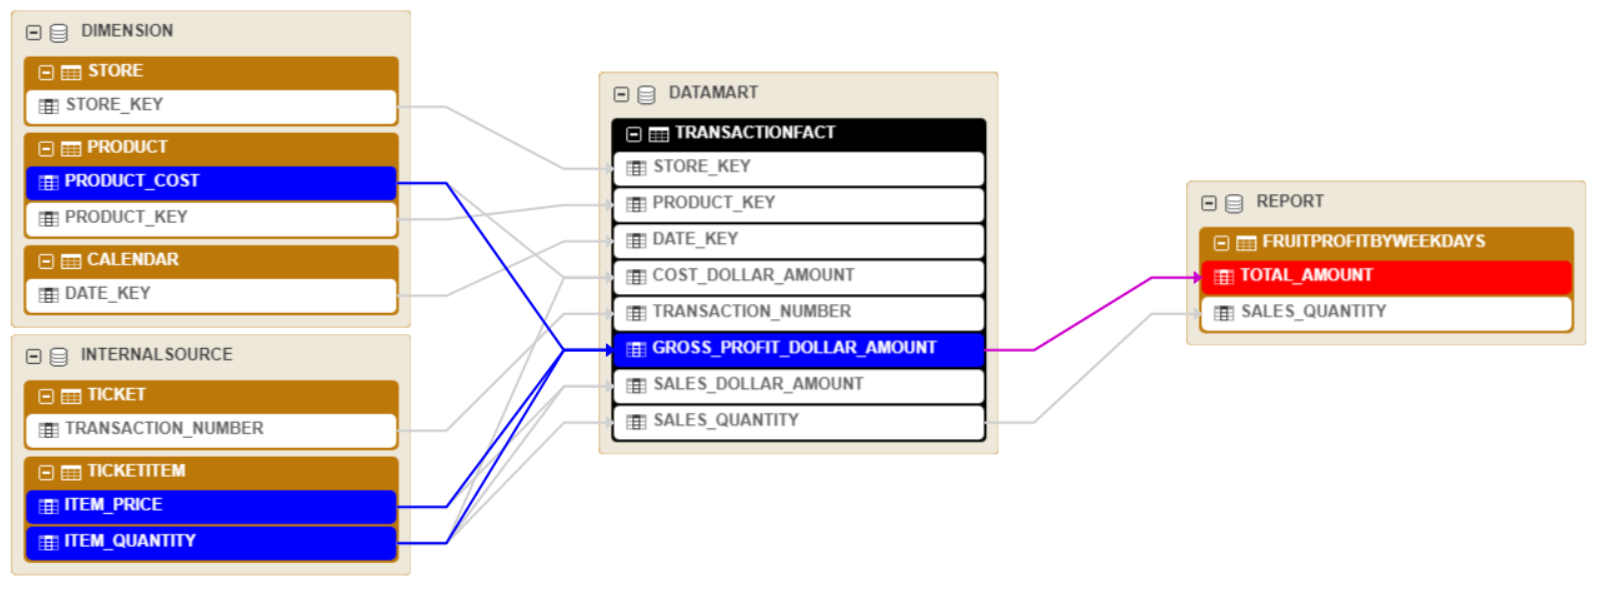
\includegraphics[width=0.8\linewidth]{img/flow_visualizace}
   \end{figure}
\end{frame}

\section{Definice problému}
\begin{frame}
\frametitle{Definice problému}
   \begin{itemize}
      \item Existuje velké množství grafových databází
      \item Jednotlivé databáze se výrazně liší ve výkonostních parametrech
      \item Oblast je dynamická, vznikají nové nástroje, končí podpora pro některé stávající
      \item Neexistují obecné standardy pro jejich dotazování
      \item To vede k silné závislosti aplikací na používané grafové databázi a dotazovacím jazyce
      \begin{itemize}
         \item Dochází k prolínání perzistentní a byznys logiky aplikace
         \item Aplikace je obtížně spravovatelná a modifikovatelná
      \end{itemize}
   \end{itemize}
\end{frame}

\section{Cíle práce}
\begin{frame}
\frametitle{Cíle práce}
   \begin{itemize}
      \item Seznámení se s grafovými databázemi a jejich API
      \item Analýza způsobu využívání grafové databáze v aplikaci \textit{Manta Flow}
      \item Identifikace omezení stávající architektury aplikace vzhledem k práci s grafovou databází
      \item Rešerše existujících nástrojů pro abstrakci grafových databází
      \item Návrh vícevrstvé architektury abstrahující práci s grafovou databází
      \item Vytvoření prototypové implementace navržené architektury
   \end{itemize}
\end{frame}

\section{Dosažené výsledky}
\begin{frame}
\frametitle{Dosažené výsledky}
   \begin{enumerate}
      \item Rešerše grafových databází a možností jejich dotazování
      \item Rešerše softwarových architektur vhodných pro návrh architektury
      \item Analýza jednotlivých komponent aplikace \textit{Manta Flow} a způsobu práce aplikace s grafovou databází
      \item Identifikace omezení aplikace plynoucích ze stávající architektury aplikace
      \item Specifikace konkrétních požadavků na navrhovanou architekturu na základě analýzy
      \item Analýza existujících nástrojů pro abstrakci grafových databází
      \seti
   \end{enumerate}
\end{frame}
\begin{frame}
\frametitle{Dosažené výsledky}
   \begin{enumerate}
      \conti
      \item Návrh vícevrstvé architektury pro práci s grafovou databází a příslušných API
      \item Prototypová implementace navržené architektury
      \item Implementace vybraných algoritmů tvořících byznys logiku aplikace pomocí prototypové implementace architektury
      \item Otestování prototypové implementace pomocí jednotkových a integračních testů
      \item Návrh úpravy architektury dalších částí aplikace na základě navržené architektury
   \end{enumerate}
\end{frame}


\section{Základní charakteristiky navržené architektury}
%------------------------------------------------
\begin{frame}
\frametitle{Základní charakteristiky navržené architektury}
   \begin{itemize}
      \item Vícevrstvá architektura - funkcionalita rozdělena do několika vrstev
      \item Definován specifický doménový model
      \item API perzistentní vrstvy vycházející z \textit{Repository patternu}
      \item Oddělené metody využívající externí indexy
      \item Deklarativní transakční model
   \end{itemize}
\end{frame}
%------------------------------------------------
\begin{frame}
\frametitle{Základní charakteristiky navržené architektury}
   \begin{figure}
   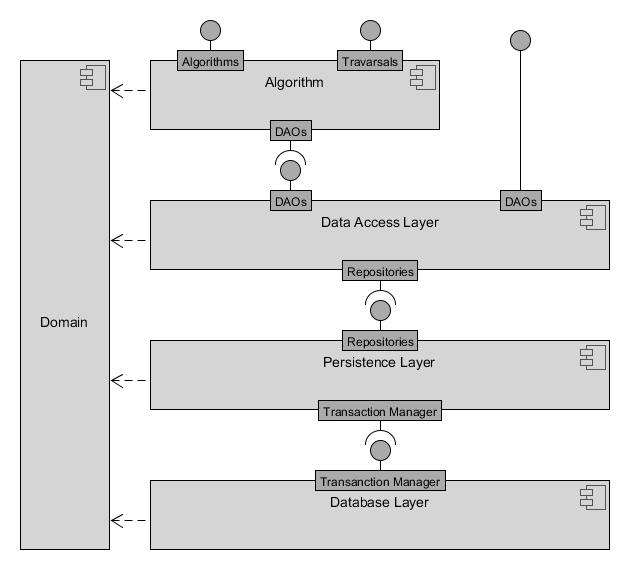
\includegraphics[width=0.7\linewidth]{img/connector_modules}
   \end{figure}
\end{frame}
%------------------------------------------------

\section{Přínosy práce}
%------------------------------------------------
\begin{frame}
\frametitle{Přínosy práce}
% TODO
\begin{itemize}
\item Je navržena vícevrstvá architektura sloužící pro přístup ke grafové databázi
\item Na základě prototypové implementace je ověřena vhodnost návrhu architektury
\item Architektura odděluje perzistentní a byznys logiku aplikace a výrazně tak zlepšuje její modifikovatlnost
\item Jsou navrženy dílčí kroky umožňující budoucí škálování aplikace
\end{itemize}
\end{frame}
%------------------------------------------------
\begin{frame}
   \centering\Large Děkuji za pozornost
   \vspace{2em}

   \centering\normalsize
   Jakub Moravec\\ jkb.moravec@gmail.com
\end{frame}


\end{document}
